\documentclass{ximera}

\author{Jenny Sheldon \& Jim Talamo}
\newcommand{\RR}{\mathbb R}
\renewcommand{\d}{\,d}
\newcommand{\dd}[2][]{\frac{d #1}{d #2}}
\renewcommand{\l}{\ell}
\newcommand{\ddx}{\frac{d}{dx}}
\newcommand{\dfn}{\textbf}
\newcommand{\eval}[1]{\bigg[ #1 \bigg]}


\title{Dig-In: Estimating Series}

\outcome{Define the remainder for a convergent series.}
\outcome{Estimate the value of a convergent series using the sequence of partial sums.}
\outcome{Explain the relationship between the remainder of a convergent series and the sequence of partial sums.}




\begin{document}
\begin{abstract}
    We learn how to estimate the value of a series.
\end{abstract}
\maketitle

Once we know that a series converges, it's incredibly useful to be able to estimate its value, especially in the context of science or engineering.  For most practical purposes, we don't need the exact value of a convergent series, but can instead compute with a replacement value that is close enough, or within a predetermined margin of error.

\begin{question}
Consider the series
\[
\sum_{n=1}^{\infty} \frac{1}{n^2}.
\]
\begin{enumerate}
    \item Does it make sense to approximate this series?
        \begin{prompt}
        \wordChoice{\choice[correct]{Yes, because the series converges.} \choice{No, because the series diverges.}}
        \end{prompt}
    \item What test is most appropriate for determining the convergence or divergence of this series?
        \begin{prompt}
        \wordChoice{\choice{The series is geometric or telescoping.} \choice[correct]{The series is a convergent $p$-series.} \choice{The divergence test.}}
        \end{prompt}
    \item Using the first four terms of this series in place of the infinite series, what value could we use to estimate the series?
        \begin{prompt}
        $\answer[given]{1 + \frac{1}{4}+ \frac{1}{9} + \frac{1}{16}}$
        \end{prompt}
\end{enumerate}

\end{question}


Also, notice that we already have language for this estimate: we called it our partial sum $s_n$.  In other words, for any convergent infinite series, we can use $s_n$ in place of the sum $S = \sum \limits_{k=1}^\infty a_k$ as an estimate.  Remember that $s_n$ is finite for any value of $n$.

Now that we have an estimate, our next question should be: just how good is that estimate, anyway?  We've made a guess, but how accurate is our guess?  Adding up a thousand terms, or ten thousand terms, or even ten million terms of a series does not necessarily give us an estimate which is within our margin of error!  This is where the idea of the remainder comes in.

\begin{definition}
Let
\[
 \sum \limits_{k=1}^\infty a_k
\]
be an infinite series which converges to $S = \sum \limits_{k=1}^\infty a_k$.  Define $r_n$, the remainder when using $s_n$ in place of $S = \sum \limits_{k=1}^\infty a_k$, or just the remainder for short, as
\[
r_n = \sum \limits_{k=n+1}^{\infty} a_k.
\]
\end{definition}

Notice that $r_n$ is also an infinite series, and that its index starts at $n+1$.  The reason for writing the starting index in this way is so that we can think of splitting up the sum $S = \sum \limits_{k=1}^\infty a_k$ into our estimate, $s_n$, and our remainder $r_n$.

\begin{image}
  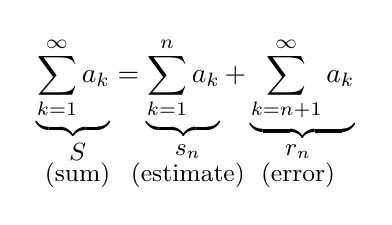
\begin{tikzpicture}
        \node at (0,0) {
           $\underbrace{\sum \limits_{k=1}^\infty a_k}  = \underbrace{\sum \limits_{k=1}^n a_k} + \underbrace{\sum \limits_{k=n+1}^\infty a_k} $ 
           };
        \node at (-0.1,-.8) {\small{$s_n$}};
        \node at (-0.1,-1.1){\small{(estimate)}};
        \node at (1.3, -.8) {\small{$r_n$}};
        \node at (1.3,-1.1) {\small{(error)}};
        \node at (-1.5, -0.8) {\small{$S$}};
        \node at (-1.5, -1.1) {\small{(sum)}};
      \end{tikzpicture}
  \end{image} %%Jim fixes this

\begin{remark}
Note that in general, we can repeat this construction in this section for any convergent series for which the lower index is $n_0$.

\begin{align*}
\sum_{k=n_0}^\infty a_k &= \sum_{k=n_0}^n a_k+\sum_{k=n+1}^\infty a_k,
\end{align*}

where $n \geq n_0$.  The remainder $r_n$ is defined by the same formula $r_n = \sum_{k=n+1}^{\infty} a_k$, but we only have remainders for $n \geq n_0$ (rather than for $n \geq 1$).  

In fact, you may have noticed that we use similar notation for the remainders $r_n$ as we do for the sequence of partial sums $\{s_n\}_{n = n_0}$.  This isn't a coincidence; we actually can define a sequence of remainders $\{r_n\}_{n=n_0}$, beginning at $n=n_0$.  In practice, however, we think of the remainders one at a time, rather than as a whole sequence. 
\end{remark}


At this point, you should test out these definitions on a geometric series where you can find concrete values for the sum, the estimate, and the error for any value of $n$.  As usual, being able to check your own work helps you to familiarize yourself with the concepts involved, and helps you to organize the various pieces involved.  In general, however, we only want to estimate series whose sum we cannot evaluate. Let's look at such an example.

\begin{example}
Consider the series
\[
\sum \limits_{n=1}^{\infty} \frac{1}{n^2}.
\]
This series converges, but $\sum_{k=1}^{\infty} \frac{1}{k^2}$ \wordChoice{\choice{is}\choice[correct]{is not}} a geometric series and is not a telescoping series.  That means we don't yet have the tools to evaluate the sum.  Instead, we will use $n=4$ to decompose the series into an estimate $s_n$ and a remainder $r_n$.

\begin{explanation}
\begin{align*}
    \sum \limits_{n=1}^\infty \frac{1}{n^2} &= \sum \limits_{n=\answer[given]{1}}^{\answer[given]{4}} \frac{1}{n^2} + \sum \limits_{n=\answer[given]{5}}^{\answer[given]{\infty}} \frac{1}{n^2} \\
    \sum \limits_{n=1}^\infty \frac{1}{n^2} &= \answer[given]{1 + \frac{1}{4} + \frac{1}{9} + \frac{1}{16}} + r_4
\end{align*}
\end{explanation}
\end{example}

\begin{remark}
Finding the exact value of the series $\sum_{k=1}^{\infty} \frac{1}{k^2}$ is not easy!  In fact, this problem was first posed by the Italian mathematician Pietro Mengoli in 1650 and became known as the Basel problem. The problem remained unsolved for nearly 100 years. In 1734, the famous mathematician Leonard Euler finally found the sum.  
\end{remark}

Generally, our goal is choose a value of $n$ that will make the remainder small.  For this reason, we will sometimes refer to the remainder as the error.  We think of $s_n$ as making up most of the sum, and then $r_n$ tells us how far $s_n$ is from the actual sum $S = \sum \limits_{k=1}^\infty a_k$.  

Since $r_n = \sum \limits_{k=n+1}^{\infty} a_k$ is still an infinite series, its exact value is hard to find.  Most of the time, then, our goal will be to find an upper bound for this error.  We then use our upper bound to guarantee that our estimate $s_n$ is a good estimate.  Of course, what it means to be a ``good'' estimate varies widely from application to application!

\begin{question}
It's true that
\[
\sum \limits_{n=1}^\infty \frac{1}{n^2}  = \frac{\pi^2}{6}.
\]
Which of the following statements are true of $r_4$ for this series?
\begin{selectAll}
\choice{$r_4$ has $4$ terms.}
\choice[correct]{$r_4 > 0$}
\choice{$r_4 > s_4$}
\choice[correct]{$r_4 < \frac{\pi^2}{6}$}
\choice[correct]{$r_4 < 1$}
\choice{$r_4 < 0.1$}
\choice{$r_4< 0.01$}
\end{selectAll}
\end{question}

Let's try a different kind of example.
\begin{example}
Suppose that $\{a_n\}_{n=1}$ is a sequence and it is known that $\sum_{k=1}^{n} a_k = \frac{2n}{n+1}$.  
\begin{enumerate}
    \item Explain why the series $\sum_{k=1}^{\infty} a_k$ converges, and why its convergence is significant towards finding the remainder.
    \item Find an explicit formula for $r_n$.
    \item Find an integer $N$ so $\sum_{k=1}^{N} a_k$ is within $.01$ of the exact value of $\sum_{k=1}^{\infty} a_k$.
\end{enumerate} 

\begin{explanation}
\begin{enumerate}
\item Note that we are actually given that $s_n = \frac{2n}{n+1}$.  Since $\lim_{n \to \infty} s_n = \answer{2}$, we have that $\sum_{k=1}^{\infty} a_k$ \wordChoice{\choice{diverges}\choice[correct]{converges to $2$}} .

Since the series \wordChoice{\choice{diverges}\choice[correct]{converges}}, it makes sense to talk about the remainder $r_n$ for any $n \geq 1$, since $r_n$ will be a finite number for each $n$.  

\item Notice that the relationship $\sum_{k=1}^{\infty} a_k = s_n+r_n$ allows us to find an explicit formula for $r_n$.
\begin{align*}
\sum_{k=1}^{\infty} a_k &= s_n+r_n \\
2 &= \frac{2n}{n+1}+r_n \\
r_n &= 2-\frac{2n}{\answer[given]{n+1}}
\end{align*}


\item This question is really asking how many terms we need in a finite sum to ensure that the computed value will be accurate to $.01$ of the exact value of the infinite series.  Since $r_N$ will measure the error resulting from approximating the infinite series by $s_N$, we find $N$ by setting $\vert r_N \vert \leq .01$.  We can choose any value of $N$ which will satisfy this property.  Let's choose to find the smallest such value of $N$, since we have a nice procedure for doing so.

\begin{align*}
2-\frac{2N}{N+1} &\leq \frac{1}{100} \\
200-\frac{200N}{N+1} & \leq 1 \\
\frac{200N}{N+1} & \geq 199 \\
200N & \geq 199N+199 \\
N \geq \answer[given]{199}
\end{align*}

We thus know that $s_{199}$ can be used to approximate the value of $\sum_{k=1}^{\infty} a_k$ to within $.01$ of its exact value.  Notice that any value of $N$ which is greater than $199$ will also satisfy this property!  To be consistent, we will often ask specifically for the smallest possible value of $N$.
\end{enumerate}
\end{explanation}

\end{example}

Another thing to notice about the previous example: since we found a formula for $r_n = 2 - \frac{2n}{n+1}$, it's easy to see that $\lim \limits_{n \to \infty} r_n = 0$. In other words, if we increase the value of $n$, we decrease the error.  Said another way, the more terms we use when approximating a convergent series, the smaller our error should be in general.  This is part of a more general statement about the relationship between converging series and their remainders.

\begin{theorem}[Remainders and Convergence]\index{remainders and convergence}
Consider the series $\sum_{k=n_0}^{\infty} a_k$ and for every $n \geq n_0$, define $r_n = \sum_{k=n+1}^{\infty} a_k$.  If $\sum \limits_{k=1}^\infty a_k$ converges, then $\lim \limits_{n \to \infty} r_n = 0$.   
\end{theorem}

This theorem hopefully makes sense: if we think of 
\[
r_n = \sum \limits_{k=1}^\infty a_k - s_n,
\]
and we take the limit as $n$ goes to infinity on both sides, we know that $\lim \limits_{n \to \infty} s_n = \sum \limits_{k=1}^\infty a_k$ by the meaning of $s_n$.  The left hand side, or $r_n$, thus can be made as small as we wish.

\section{Summary}
Overall, there are two main types of questions we would like to answer about remainders.
\begin{enumerate}
    \item What is the error involved with using a specified number of terms?
    \item How many terms of a series (what is the value of $n$) should we use to obtain a desired precision?
\end{enumerate}

While they are worded similarly, the two questions describe different situations in which we might find ourselves.  In the first, we want to add a specified number of terms - perhaps due to limitations in technology, memory space, or time.  Remember - estimating the error is a practical matter!  In the second, we want to achieve a specified precision, or make the error smaller than some specified threshold.  Again, in any practical circumstance, the threshold will likely be decided by safety specifications, sensitivity of instrumentation, or a required number of significant figures.  Of course, in the controlled classroom environment, such a threshold will be given.  But in a professional environment, the choice will likely be yours.

Look back again over the examples we solved together in this section.  We've worked through problems of both of these types, and we will continue to do so throughout the upcoming sections.

\end{document}